% !TeX root = ../main.tex
\documentclass[tikz]{standalone}
\usepackage{pgfplots}
\pgfplotsset{compat=newest}
\begin{document}
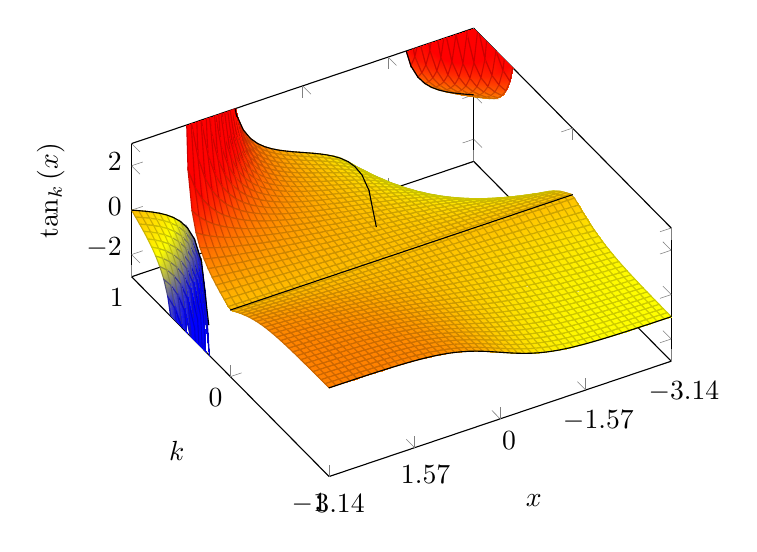
\begin{tikzpicture}[
        declare function={
                tangent(\x,\y)= (\x>=0) * tan(\x*deg(\y)) + (\x<0) * tanh(-\x*\y);
            },
    ]
    \begin{axis}[
            colormap/hot,
            xlabel = \(k\),
            ylabel = \(x\),
            zlabel = \(\tan_k\left(x\right)\),
            domain=-1:1,
            domain y = -pi:+pi,
            ytick = {-pi,-pi/2,0,+pi/2,+pi},
            zmin = -3,
            zmax = +3,
            restrict z to domain = -9:+30,
            point meta min = -3,
            point meta max = +3,
            view = {240}{60},
            samples = 50,
        ]
        \addplot3 [
            surf,
            shader = faceted interp,
        ] {tangent(\x,\y)};
        \addplot3 [
            black,
            smooth,
        ](0, \y, 0);
        \addplot3 [
            black,
            smooth,
        ](1, \y, {tan(deg(\y))});
        \addplot3 [
            black,
            smooth,
        ](-1, \y, {tanh(\y)});
    \end{axis}
\end{tikzpicture}
\end{document}